\subsubsection{Local data Capture}		 
The following use cases pertain to how Condenser records data local to it. Figure~\ref{LocalDataCaptureUse} shows a diagram depicting the relationships between the local data capture use cases.
\begin{center}
	\begin{figure}[htbp]
		%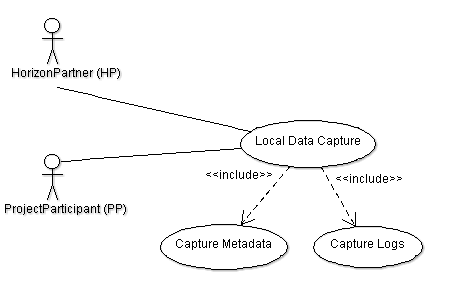
\includegraphics[scale=.75]{images/LocalDataCaptureUse.png}
		\caption{Use cases defining Condenser local data capture. \label{LocalDataCaptureUse}}
	\end{figure}
\end{center}	
\textbf{Use Cases:}\\

		\textbf{Capture Data}\\	 
		\textbf{Participating Actors:} Horizon Partner (HP) and/or Project Participant(PP) \\
		\textbf{Event Flow:}
		\begin{enumerate}
\item The HP or PP initiates data transfer from one or more nodes to Condenser.
\item As Condenser receives data from its subscriptions, it stores the data and metadata (see Capture Metadata use case) to its database.
\item Condenser logs activity as per its logging settings  (see Capture  Logging Information use case) .
	    \end{enumerate}
		\textbf{Entry Conditions:} Condenser is installed in an environment and nodes are registered with it.\\
		\textbf{Exit Conditions:} Condenser is recording (and possibly transferring) one or more data streams.\\
		\textbf{Quality Requirements:} 
		\begin{itemize}
\item Stored data is time stamped and connected to appropriate metadata.
\item Condenser should offer a high degree of reliability regarding data transfers to it (very little to no data loss)
\item Condenser should be able to handle receiving secure (encrypted) and unsecured data streams.
		\end{itemize}
		\line(1,0){350}	
		
		\textbf{Capture Metadata}\\	 
		\textbf{Participating Actors:} Horizon Partner (HP) and/or Project Participant(PP) \\
		\textbf{Event Flow:}
		\begin{enumerate}
\item Data streams begin to provide data points when the HP or PP initiate data transfer.
\item Each data point is captured in the database along with provenance metadata such as time stamps. Some of these metadata points will be links to descriptive records.
	    \end{enumerate}
		\textbf{Entry Conditions:} Metadata pertaining to given nodes was registered at time of node subscription.\\
		\textbf{Exit Conditions:} Node data is described appropriately.\\
		\textbf{Quality Requirements:} Metadata writing should not interfere with node data capture reliability. \\
		\line(1,0){350}	
		
		\textbf{Capture Logging Information}\\
		\textbf{Participating Actors:} Horizon Partner (HP) and/or Project Participant(PP) \\
		\textbf{Event Flow:}
		\begin{enumerate}
\item Data streams begin to provide data points when the HP or PP initiate data transfer.
\item Condenser should make log recordings of events such as error conditions within its own recording and/or transmission schemes, or anomalous node behaviour (such as if nodes go offline unexpectedly).
	    \end{enumerate}
		\textbf{Entry Conditions:} Logging is set up to at a sufficient level of verbosity.\\
		\textbf{Exit Conditions:} Log records can be made of events.\\
		\textbf{Quality Requirements:} Log writing should not interfere with node data capture reliability. \\
		\line(1,0){350}	